\documentclass[12pt, letterpaper]{article}
\usepackage[utf8]{inputenc}
 \usepackage[letterpaper, margin=0.8in]{geometry}
 \usepackage{amssymb}
\usepackage{amsmath}
 \usepackage{enumitem}
\usepackage {listings}
\usepackage{pgfplots}
\usepgfplotslibrary{external}
\usepackage{graphicx}

\title{CS425 Project 3(Report)\\k-Nearest-Neighbors and Decision Trees}
\author{Ksenia Burova}
\date{November \(6^{th}\), 2017}

\begin{document}
\maketitle

{\noindent {\bf Abstract:} In machine learning, k-Nearest-Neighbors (kNN) algorithm is one of the nonparametric estimation methods, and in nonparametric methods we assume that similar data inputs have similar data outputs. In this project, we were given data file with different attributes that correspond to breast cancer diagnosis. The goal of the project was to run both, kNN and Decision Trees algorithms, to see how well they perform in predicting a tumor being benign or malignant. There were several performance metrics to be used to analyze results. Some of those metrics were displayed in plots. \\}

\begin{enumerate}[label=\Roman*.]
	
	{\bf \item Project Data.} \\
	
	 In this project, we were given a file {\it breast-cancer-wisconsin.data} which had 11 attributes:
	 \begin{enumerate}[label=\arabic*.]
	 	\item Sample code number: id number
		\item Uniformity of cell size: 1 - 10
		\item Uniformity of Cell Shape: 1 - 10
		\item Marginal Adhesion: 1 - 10
		\item Single Epithelial Cell Size: 1 - 10
		\item Bare Nuclei: 1 - 10
		\item Bland Chromatin: 1 - 10
		\item Normal Nucleoli: 1 - 10
		\item Mitoses: 1 - 10
		\item Class: (2 for benign, 4 for malignant)
	\end{enumerate}
	
	I removed a column with {\bf id number}  since it is not relevant in predicting tumor type. There were also some data with missing values. My choice was not to predict those values, instead, I excluded that data from the data set. I decided to use such method to avoid incorrect prediction that may influence experiment results. \\
	
	I've placed all continuous values for this data into multidimensional array called {\bf dataFeatures}, and kept classes in one-dimensional array called {\bf dataLabels} for simplicity of implementation. \\
	During experiments, data was split into 3 sets: training, validation and testing. First I've split the whole data into training and testing data sets with 70/30 proportion rule. Then training data was divided into training and validation parts with 70/30 proportion rule as well for cross validation purposes. \\
	
	{\bf \item Tools and Program.}\\
	
	I've used {\bf python} programming language, {\bf numpy} library for arithmetic, {\bf sklearn} library for splitting my data into training, validation and testing datasets, and {\bf matplotlib} library to built plots for this project. I have a program named {\bf knn-dt.py} , that includes implementation of both parts of the project. I've split each algorithm into several functions for efficiency, and in the very end of my program I do main calls to run experiments and build plots.\\
	
	{\bf \item Performance metrics.}\\
	
	To evaluate performance of  classification algorithms, we have to compare correct classifications with our classifications on evaluation data sets after algorithm is run. We are going to calculate and look at the following values: 
	\begin{itemize}
		\item Confusion Matrix \\
		
		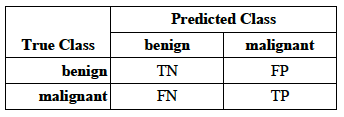
\includegraphics[scale=0.7]{../images/1.png} \\
		where TP = \# true positives, TN = \# true negatives, FP = \# false positives, FN = \# false negatives.\\
		
		\item Accuracy = (TN + TP) / (TN + TP + FN + FP)\\
		Accuracy tells us how what percent of data what classified correctly. \\
		\item TPR (true positive rate, recall, or sensitivity) = TP / (TP + FN)\\
		\item PPV (positive predictive value or precision) = TP / (TP + FP)\\
		\item TNR (true negative rate or specificity) = TN / (TN + FP)\\
		\item F Score = PPV * TPR / (PPV + TPR)\\
	\end{itemize}
	
	{\bf \item Part 1. k-Nearest-Neighbors. }\\
	
	kNN algorithm, as all nonparametric algorithms, is composed of finding the similar instances from the training set using one of distance measures and interpolating from them to find the right output. Distance measures may differ but in our experiment we are going to use Euclidian distance between two multidimensional data points:\\
	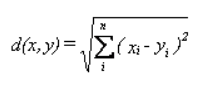
\includegraphics[scale=0.7]{../images/d1.png} 
	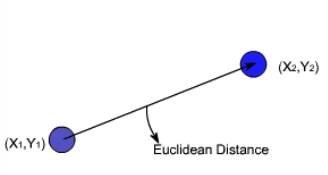
\includegraphics[scale=0.5]{../images/d2.png} 
	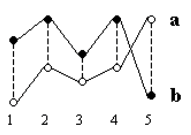
\includegraphics[scale=0.7]{../images/d3.png} \\
	
	\begin{enumerate}[label=\arabic*.]

	\item {\it Calculating Neighborhood. }\\
	The first part of the algorithm after splitting datasets, is to calculate distances for each evaluation(validation or testing) data point and all data points in training set. After that we choose k data points from training set which become k nearest neighbors, obviously. So, our neighborhood for each evaluation data point consists of training data points that are the closest distance-wise. We've used different values of k in this project to compare performance and determine the best ones. The values were following: 2, 3, 4, 5, 6, 7, 8, 16, 32.\\
	
	\item {\it Classification. }\\
	When neighborhood is known for each  evaluation data point, we can classify those data points. What we do is counting votes of each neighbor for class and choose class with the maximum number of votes. For example, if we have three neighbors and two of them are benign and one is malignant, that means that two neighbors vote for class '2', and one votes for class '4'. Since we have more votes for class '2', our evaluation data point will be classified as benign. There are ties possible, in this case I always make evaluation data point to be classified as malignant. Not only it's the one of the most common ties resolutions, in my mind, it makes sense. If we can't be really positive on tumor being good it's better to mark it as bad. \\
	
	\item {\it Performance. }\\
	After we are done with the major part of algorithm, we have to run it for multiple k values to determine the most optimal one. Before we run kNN for all values, we split training set into training and validation parts. We predict classification for validation set and compare them with real values. For performance metrics, we use confusion matrix that records number of true-positive, true-negative, false-positive and false-negative value. Using metrics from confusion matrix, we calculate prediction accuracy and other relevant measurements of performance. \\
	
	Results for k = 2, 3, 4, 5, 6, 7, 8, 16, 32 look as following: \\
	
	\begin{center}
	 	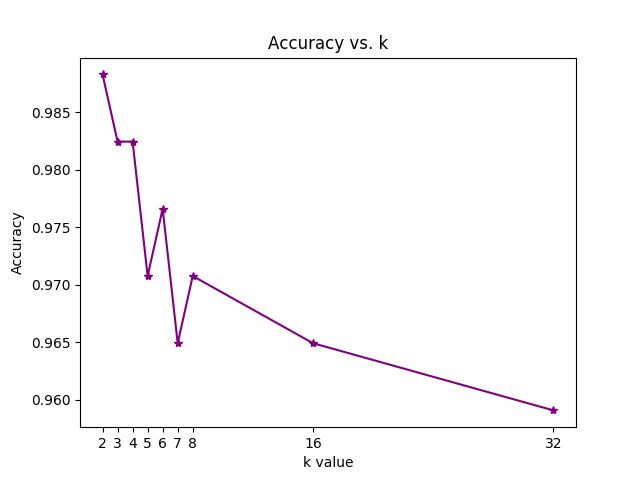
\includegraphics[scale=0.7]{../images/accuracy.png} 
	\end{center}
	\end{enumerate}
	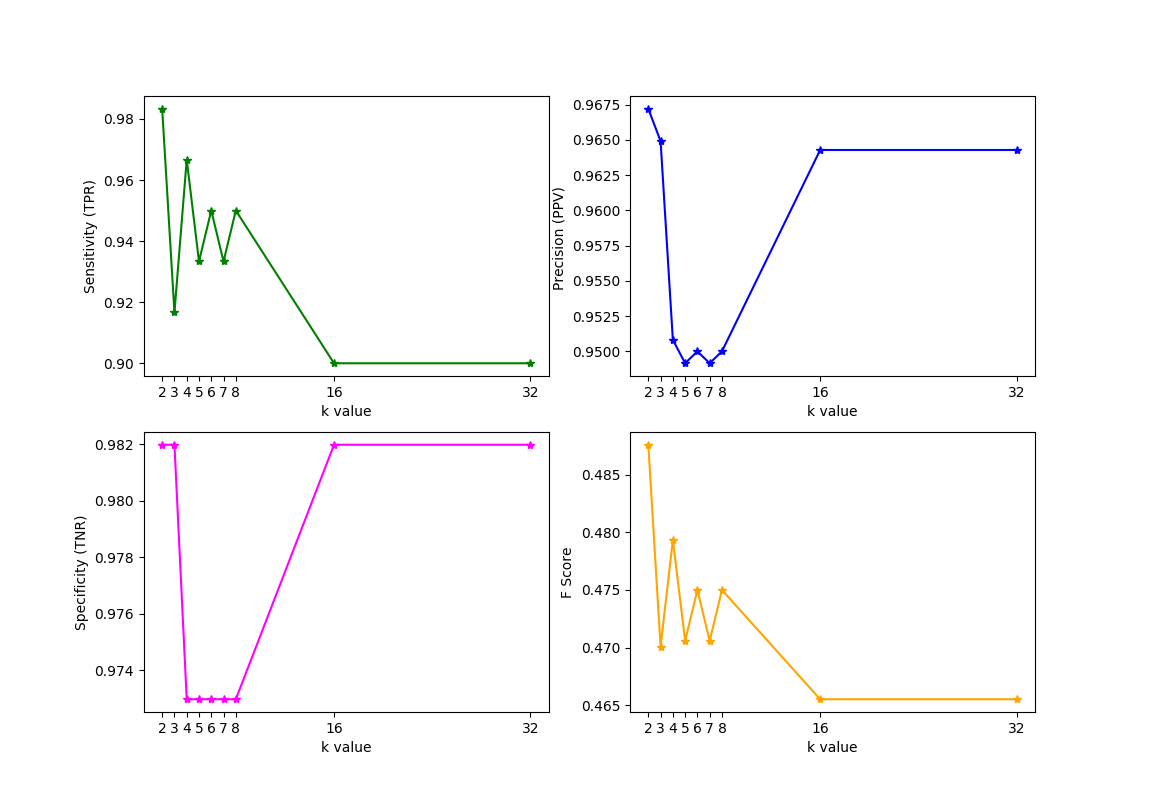
\includegraphics[scale=0.65]{../images/metrics.png} 

	
	{\bf \item Part 2. Decision Trees. }\\
	
	{\bf \item Conclusions.}\\
	  
	  
\end{enumerate}
	
	
	
	
	
	
	
\end{document} 